% ARR / *ACL submission -- ANONYMOUS REVIEW VERSION
% Build:  latexmk -pdf paper.tex
% Switch to camera-ready by changing [review] to [] in \usepackage{acl}.
\documentclass[11pt]{article}

\usepackage[review]{acl}

\usepackage{times}
\usepackage{latexsym}
\usepackage[T1]{fontenc}
\usepackage[utf8]{inputenc}
\usepackage{microtype}
\usepackage{graphicx}
\usepackage{booktabs}
\usepackage{amsmath}
\usepackage{csquotes}
\usepackage[capitalise]{cleveref}

\graphicspath{{../figures/}}

\newcommand{\Zcurr}{\ensuremath{Z_{\mathrm{curr}}}}

\title{Effective, Specific, and Non-Selective: Activation Interventions on
       Sequentially Computed State}

\author{Anonymous ARR submission}

\begin{document}
\maketitle

\begin{abstract}
Interpretability research increasingly validates activation interventions by
showing that they produce an intended counterfactual answer. RAVEL established
that this is insufficient for static entity attributes: a faithful
intervention must also leave unrelated attributes intact, and MIB reports that
full-vector interventions fail exactly this test. We ask whether the same
distinction holds when the target is not a stored attribute but a state
computed over several reasoning steps. Using a transfer task with a known
causal program ($\mathrm{holder}_{t+1} = \mathrm{recipient}_t$), we construct
an intervention that passes a progressively strengthened battery of controls:
it changes the answer, it is specific to the donor whose state was
transplanted ($\mathrm{DS} = +0.718$, with non-injected donors at $0.000$), it
is inert under a norm-matched random direction at every magnitude, and it is
graded in magnitude. We then query the same intervened forward pass about
quantities the causal program says must not change. Selectivity is 0/240 in
two model families (95\% CI $[0.0, 1.6]$\%). Phi-3.5-mini answers
\enquote{which object moved?} with 100\% accuracy unintervened, and with a
person's name afterwards. Behavioral control of a reasoning answer does not
imply control of the reasoning state.
\end{abstract}

\section{Introduction}
\label{sec:introduction}

Activation interventions are usually validated by a single output: patch a
representation, observe the counterfactually correct answer, conclude the
representation carried the variable of interest. Interchange-intervention
accuracy formalizes this as output agreement with a high-level causal
model~\citep{geiger2021causalabstraction}.

RAVEL~\citep{huang2024ravel} showed this is only half the requirement, at
least for static entity attributes: intervening on a city's continent should
change the continent answer \emph{and leave the language answer alone}.
MIB~\citep{mueller2025mib} builds this into a benchmark and reports that
full-vector baselines do poorly on RAVEL precisely because swapping a whole
vector disturbs unrelated attributes.

Both concern attributes the model \emph{retrieves} --- a city's continent is
static, present because the entity was mentioned. We ask whether the same
distinction holds when the target is a state the model must \emph{compute}: a
value in no single input token, defined only after several reasoning steps.

Our contribution is an extension, not a new method or a new diagnostic:
RAVEL's effectiveness/selectivity distinction survives the move from static
attributes to sequentially computed state, and an intervention passing a
control battery substantially stronger than \enquote{the answer changed} still
fails it completely.

We do not claim selective interventions on reasoning state are impossible,
that interchange-intervention accuracy is invalid, or that existing methods
choose sites carelessly --- DAS~\citep{geiger2024das} restricts NLI
interventions to \texttt{[CLS]}; MIB brute-forces manually selected locations.
This is a counterexample in a controlled setting, bounded accordingly in
\cref{sec:discussion}.

\paragraph{Relation to activation steering.}
A parallel literature adds learned directions to hidden states to control
behavior, and validates them behaviorally. Our result bears directly on that
practice: a direction can produce graded, specific, norm-controlled behavioral
change while leaving the intended semantic variable untouched, so behavioral
validation alone does not license a semantic interpretation of the direction.

\section{Task: a sequentially computed causal variable}
\label{sec:task}

We use a transfer task in which objects pass between people:

\begin{quote}\small\ttfamily
Ava has the ring. Liam has the book.\\
Ava gives the ring to Emma. Liam gives the book to Henry.\\
Emma gives the ring to Owen. Henry gives the book to Grace.\\
Who has the ring? $\rightarrow$ Owen
\end{quote}

\noindent The causal program is explicit:
\begin{align*}
  \mathrm{holder}_0     &= \text{initial holder in the first sentence}\\
  \mathrm{holder}_{t+1} &= \mathrm{recipient}_t\\
  \Zcurr                &= \mathrm{holder}_k \text{ after } k \text{ transfers}
\end{align*}

Three properties make this a usable testbed.

\begin{description}
  \item[The target is computed, not retrieved] \Zcurr{} is not a property of
    any entity in the prompt; it is the result of following a chain. A recency
    heuristic fails by construction, because each round ends with a
    \emph{distractor} transfer, so the most recently named person never holds
    the queried object.
  \item[One body, several variables] Over one unchanged chain we can query the
    current holder, the last recipient, the original holder
    ($\mathrm{holder}_0$), the identity of the transferred object, and the
    number of transfers. The causal program says an intervention setting
    \Zcurr{} must change the first two and must not change the last three.
    This yields a \emph{predicted consequence pattern} rather than a single
    expected answer.
  \item[Vocabulary is controlled] Names and objects are drawn from pools
    filtered so every answer is a single token in both tokenizers, checked
    against the in-context form rather than a naive leading-space form, which
    SentencePiece splits. Donor and receiver items use disjoint names and
    objects, so a successfully transported answer is a token absent from the
    receiver's own context and cannot be explained by its surface content.
\end{description}

\section{Intervention protocol}
\label{sec:protocol}

Let $h_D$ and $h_R$ be the residual-stream activations of a donor and a
receiver at layers $L = [18, 20, 22, 24]$, at the final pre-answer token
position. The intervention adds
\[
  v = \alpha \cdot (h_D - h_R)
\]
to the receiver's activations at those layers and that position, with
$\alpha = 1$ unless stated. At $\alpha = 1$ this is exact replacement of the
receiver's state with the donor's.

\begin{description}
  \item[Position] The final pre-answer token was selected empirically before
    any held-out item was scored, and the choice is consequential: at the
    mid-sentence recipient-name position the same oracle intervention scored
    0/8, while at the final position it scored 6/8 with the identical layer
    set. A position sweep (\cref{sec:supporting}) finds effects \emph{only} at
    the final position.
  \item[Few-shot prefix] Every prompt carries a few-shot prefix covering all
    five question forms, so no probe is disadvantaged by unfamiliar formatting
    and priming is identical across conditions. This matters: with a two-form
    prefix the current-holder transport rate was 24/24; under the five-form
    prefix it is 74.2\%. We report the harder number.
  \item[Donor question] The donor prompt always ends with \enquote{Who has the
    \{object\}?}, so its final-token state corresponds to
    $do(\Zcurr := z'_D)$. That single state is then patched into receivers
    asked \emph{different} questions. This is what makes the consequence
    pattern measurable.
\end{description}

\section{The control stack}
\label{sec:controls}

Before testing selectivity we establish that the intervention is worth taking
seriously. Each control is progressively harder to pass.

\paragraph{Effectiveness.}
The patched receiver produces the donor's answer. On Phi-3.5-mini, 74.2\%
$[65.7, 81.2]$ on the current-holder probe.

\paragraph{Donor specificity.}
Measured as a cross-term \emph{within a single patched pass}, not by comparing
two separate interventions (\cref{tab:specificity}). $\mathrm{DS_{cross}} =
+0.718$. Top-1 is the injected donor 13/16; top-1 is a non-injected donor
0/16. The output tracks \emph{which} donor was supplied and does not drift
toward arbitrary names.

\begin{table}[t]
  \centering\small
  \begin{tabular}{lrr}
    \toprule
    quantity & baseline & after $do(D)$ \\
    \midrule
    $P(Y_{\text{donor}})$, injected     & 0.000 & \textbf{0.718} \\
    $P(Y_{\text{other}})$, not injected & 0.066 & \textbf{0.000} \\
    $P(Y_{\text{receiver}})$, own answer& 0.604 & \textbf{0.000} \\
    \bottomrule
  \end{tabular}
  \caption{Donor specificity as a cross-term within one patched forward pass.}
  \label{tab:specificity}
\end{table}

\paragraph{A measurement correction worth recording.}
We initially compared \enquote{patch $D \rightarrow P(Y_D)$} against
\enquote{patch a random donor $R \rightarrow P(Y_R)$}, found both succeeded at
similar rates (75\% vs 72\%), and read this as absence of specificity. That
inference is wrong: both are legitimate interchange interventions with
different donors, and the causal model predicts both should succeed. A random
donor is not a control that ought to fail. Specificity must be a cross-term
within one pass. We also verified that the near-equality was not driven by
label collision (2/32 items had a random donor whose answer coincided with the
correct donor's; enforcing a collision-free derangement left the result
unchanged) and that a true no-op self-patch reproduces the baseline exactly
32/32.

\paragraph{Norm control.}
A Gaussian direction rescaled to \emph{exactly} the norm of $h_D - h_R$
produces a change in $P(Y_{\text{donor}})$ of \textbf{0.000 at every}
$\boldsymbol{\alpha}$. The effect requires a genuine model-state direction;
injected magnitude alone does nothing.

\paragraph{Dose response.}
$P(Y_{\text{donor}})$ rises smoothly with $\alpha$ --- 0.005, 0.201, 0.601,
0.653, 0.718 at $\alpha = 0.125, 0.25, 0.5, 0.75, 1.0$ --- with a threshold
near $\alpha \approx 0.25$. The effect is graded, not an unstable
all-or-nothing flip.

\begin{figure*}[t]
  \centering
  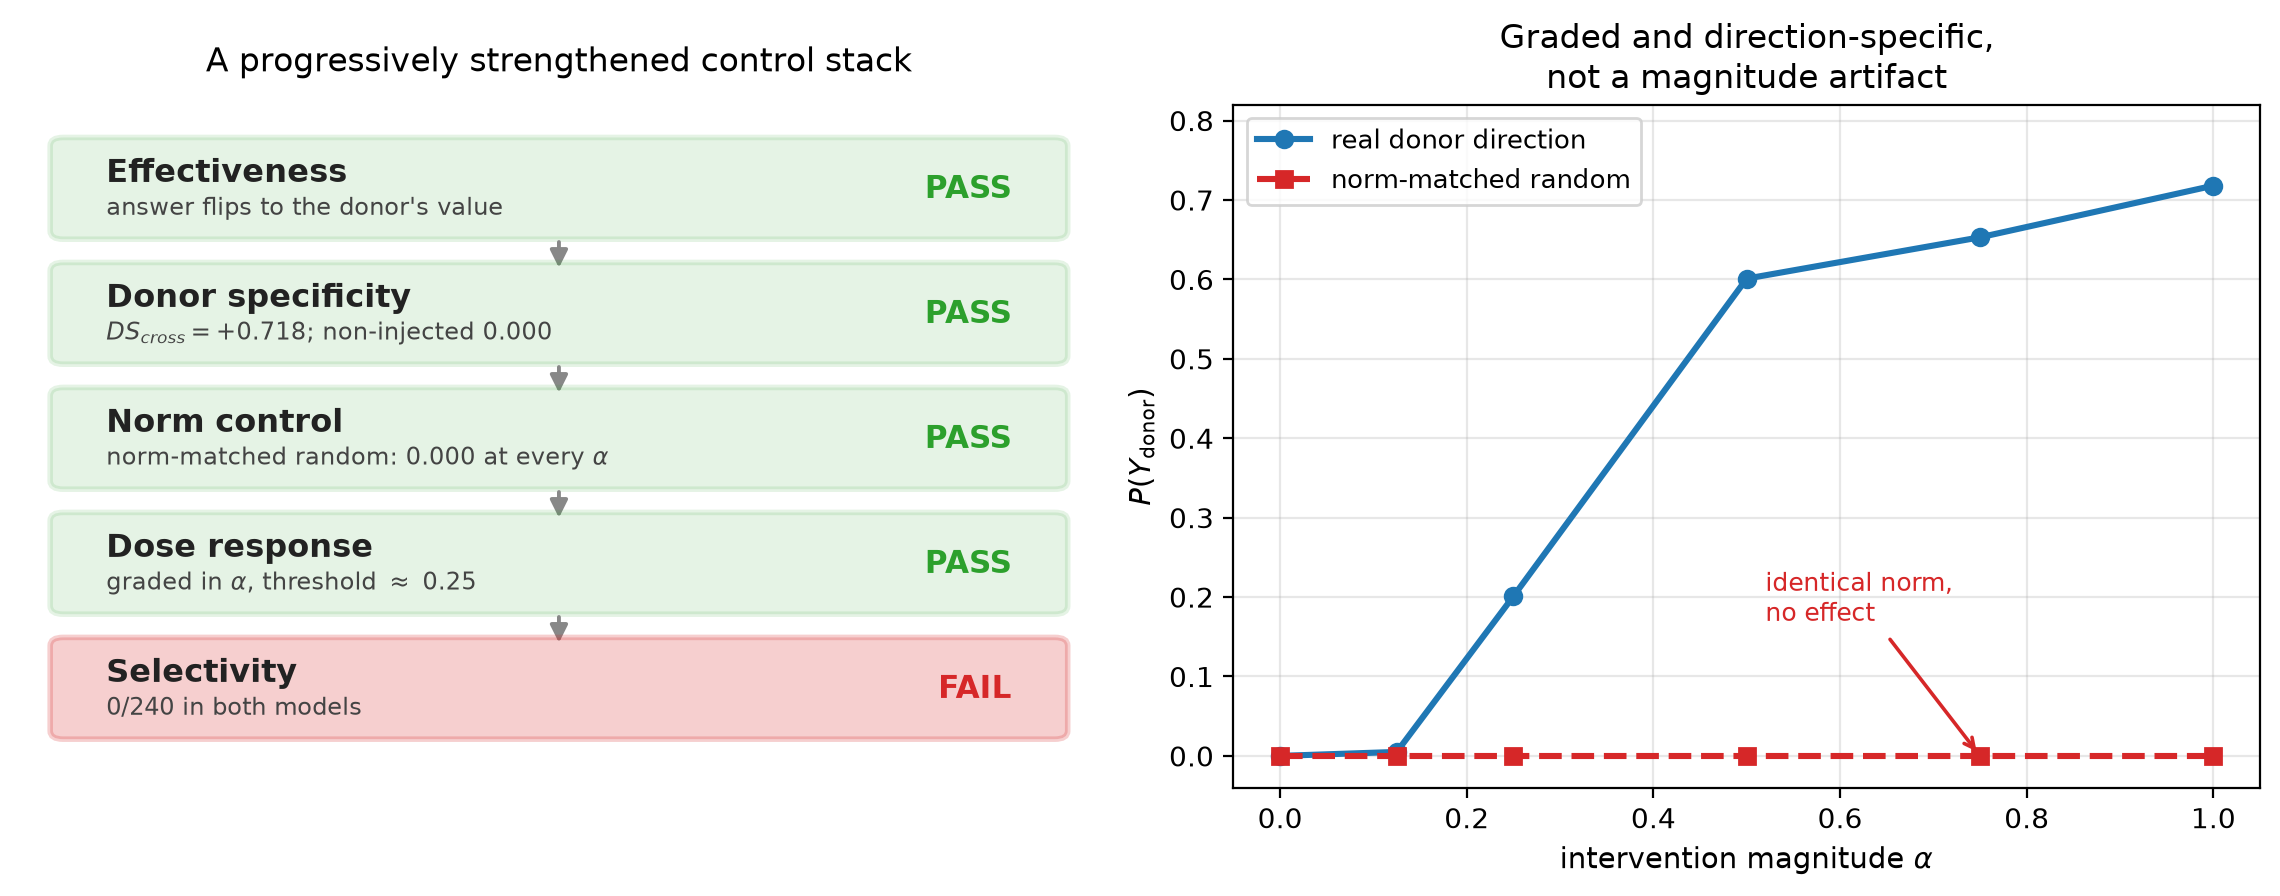
\includegraphics[width=\textwidth]{fig1_control_stack.png}
  \caption{Left: each credential in the control stack, in the order applied.
    Right: the intervention is graded in magnitude, while a direction with
    identical norm produces no effect at any magnitude.}
  \label{fig:control-stack}
\end{figure*}

\section{Selectivity evaluation}
\label{sec:selectivity}

The donor state is patched into receivers asked each of five probes. The
causal program predicts which must change (\cref{tab:probes}).

\begin{table}[t]
  \centering\small
  \begin{tabular}{llc}
    \toprule
    probe & question & change? \\
    \midrule
    \texttt{current\_holder}  & Who has the \{obj\}?        & YES \\
    \texttt{last\_recipient}  & Who received it last?       & YES \\
    \texttt{original\_holder} & Who originally had it?      & NO \\
    \texttt{object\_identity} & What object did X have?     & NO \\
    \texttt{transfer\_count}  & How many times given away?  & NO \\
    \bottomrule
  \end{tabular}
  \caption{The five probes over one unchanged chain body. YES means the probe
    must take the donor's value; NO means it must retain the receiver's.}
  \label{tab:probes}
\end{table}

\paragraph{Competence gate.}
A selectivity failure is only interpretable on probes the model can answer
\emph{unintervened}. Probes below 50\% baseline competence are excluded,
because a post-intervention change on a question the model could never answer
tells us nothing.

\paragraph{Sampling.}
3 seeds $\times$ 40 pairs $=$ \textbf{120 independent pairs per model}. Each
seed resamples both the item pairs \emph{and} the few-shot prefix. The
intervention itself is deterministic --- zero-initialized, \texttt{eval()}
mode, no optimizer --- so pairs and prefix are the only stochastic components,
and the prefix is a genuine confound worth varying. Wilson 95\% intervals are
computed over independent pairs within each probe, never over pooled
probe-outcomes.

\subsection{Phi-3.5-mini (primary)}
\label{sec:phi}

\begin{table}[t]
  \centering\small
  \setlength{\tabcolsep}{4pt}
  \begin{tabular}{llrrr}
    \toprule
    probe & chg? & baseline & $\rightarrow$don & $\rightarrow$rec \\
    \midrule
    \texttt{curr\_holder} & Y & 99.2 & 74.2 & \textbf{0/120} \\
    \texttt{last\_recip}  & Y & 97.5 & 69.2 & \textbf{0/120} \\
    \texttt{orig\_holder} & N & 100.0 & 60.0 & \textbf{0/120} \\
    \texttt{obj\_identity}& N & 100.0 & 71.7 & \textbf{0/120} \\
    \texttt{xfer\_count}  & N & 20.8\rlap{$^\ast$} & 85.8 & 0/120 \\
    \bottomrule
  \end{tabular}
  \caption{Phi-3.5-mini, percentages. $^\ast$excluded by the competence gate.
    Completeness 172/240 $=$ 71.7\% $[65.7, 77.0]$; selectivity 0/240 $=$
    \textbf{0.0\%} $[0.0, 1.6]$. Per-seed selectivity: 0/40, 0/40, 0/40.}
  \label{tab:phi}
\end{table}

\subsection{Llama-3.2-3B (corroborates selectivity only)}
\label{sec:llama}

\begin{table}[t]
  \centering\small
  \setlength{\tabcolsep}{4pt}
  \begin{tabular}{llrrr}
    \toprule
    probe & chg? & baseline & $\rightarrow$don & $\rightarrow$rec \\
    \midrule
    \texttt{curr\_holder} & Y & 46.7\rlap{$^\ast$} & 50.0 & 0/120 \\
    \texttt{last\_recip}  & Y & 73.3 & 44.2 & \textbf{0/120} \\
    \texttt{orig\_holder} & N & 100.0 & 46.7 & \textbf{0/120} \\
    \texttt{obj\_identity}& N & 100.0 & 49.2 & \textbf{0/120} \\
    \texttt{xfer\_count}  & N & 18.3\rlap{$^\ast$} & 49.2 & 0/120 \\
    \bottomrule
  \end{tabular}
  \caption{Llama-3.2-3B, percentages. $^\ast$excluded by the competence gate.
    Completeness 53/120 $=$ 44.2\% $[35.6, 53.1]$; selectivity 0/240 $=$
    \textbf{0.0\%} $[0.0, 1.6]$.}
  \label{tab:llama}
\end{table}

Llama's completeness is \emph{not} comparable to Phi's, and we do not present
it as such. Llama graded three probes; Phi graded four, because Llama's
current-holder probe fell below the competence gate at 46.7\%. Llama cannot
reliably perform the primary task at this sample size, so it supports the
\emph{selectivity} claim --- where both its graded should-not-change probes
have 100\% baseline competence --- and not the completeness claim.

\subsection{Is the metric capable of firing?}
\label{sec:metric-validation}

A counter that always reads zero is indistinguishable from a broken counter,
so we verify the instrument directly. The selectivity check and the baseline
competence check are \emph{the same comparison against the same target token},
differing only in whether the patch is applied. So the 100\% baseline
competence on \texttt{original\_holder} and \texttt{object\_identity} already
demonstrates that the selectivity check fires at ceiling when nothing is
patched. We confirm this empirically in a single process on identical items
($n=40$ per probe, both models):

\begin{table}[h]
  \centering\small
  \begin{tabular}{lrr}
    \toprule
    model & zero patch & donor patch \\
    \midrule
    Phi-3.5-mini & \textbf{80/80} & \textbf{0/80} \\
    Llama-3.2-3B & \textbf{80/80} & \textbf{0/80} \\
    \bottomrule
  \end{tabular}
  \caption{Only the patch differs. The metric is live in both models, and the
    intervention alone drives it to zero.}
  \label{tab:metric-validation}
\end{table}

The same runs show where the probability mass goes: the model answers with the
\emph{donor's} value on 21/40 and 26/40 items (Phi), 19/40 and 21/40 (Llama),
for \texttt{original\_holder} and \texttt{object\_identity} respectively.

\begin{figure}[t]
  \centering
  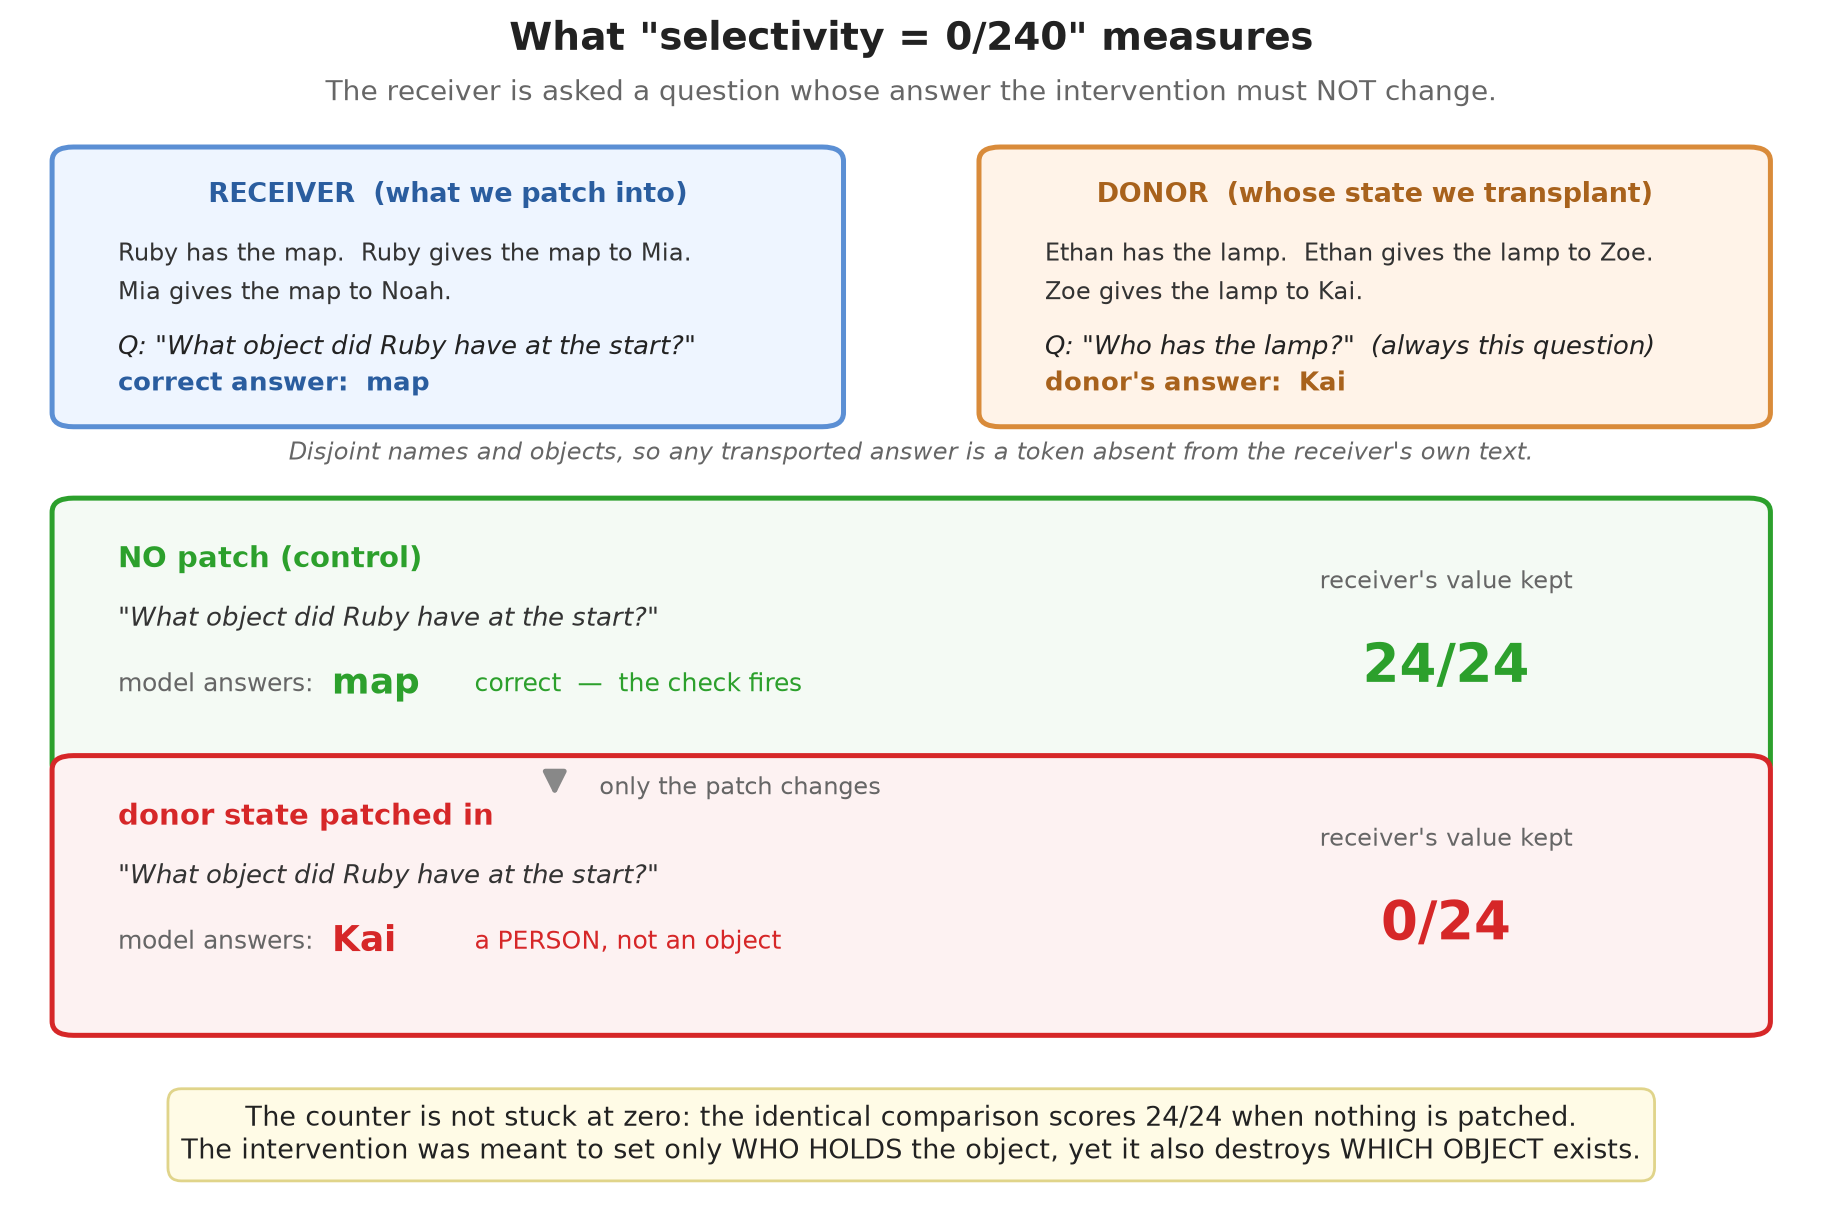
\includegraphics[width=\columnwidth]{fig4_what_selectivity_means.png}
  \caption{What the selectivity counter counts. The identical comparison
    scores 24/24 with no intervention and 0/24 with the donor patch; only the
    patch differs, so the zero reflects the intervention rather than a metric
    that cannot fire.}
  \label{fig:what-selectivity-means}
\end{figure}

\subsection{The concrete failure}
\label{sec:concrete-failure}

Both models answer \enquote{What object did \{first\} have at the start?} with
\textbf{100\% accuracy unintervened}. After an intervention that, by
construction, sets only who currently holds the object, Phi answers with a
\textbf{person's name} on 71.7\% of items. No reading of $do(\Zcurr := z'_D)$
permits changing which object exists in the problem.

This is difficult to attribute to misunderstanding the question: the model
answered it perfectly moments earlier. The intervention destroyed the semantic
isolation between the targeted answer state and unrelated information.

\begin{figure}[t]
  \centering
  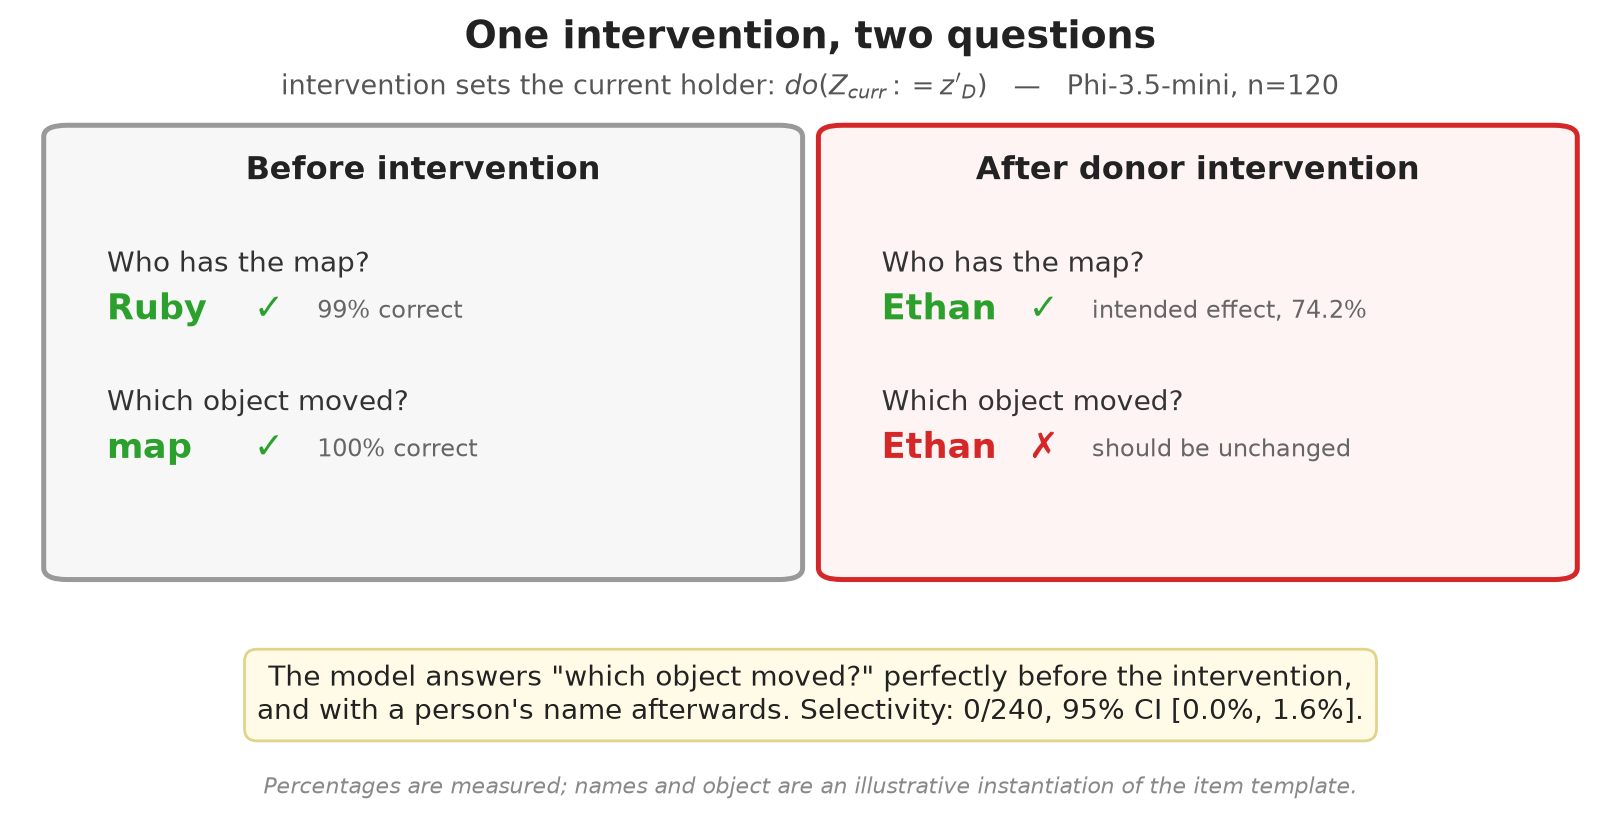
\includegraphics[width=\columnwidth]{fig2_semantic_failure.png}
  \caption{One intervention, two questions. The object-identity question is
    answered perfectly unintervened and with a person's name afterwards.
    Percentages are measured; names and object are an illustrative
    instantiation of the item template.}
  \label{fig:semantic-failure}
\end{figure}

\begin{figure}[t]
  \centering
  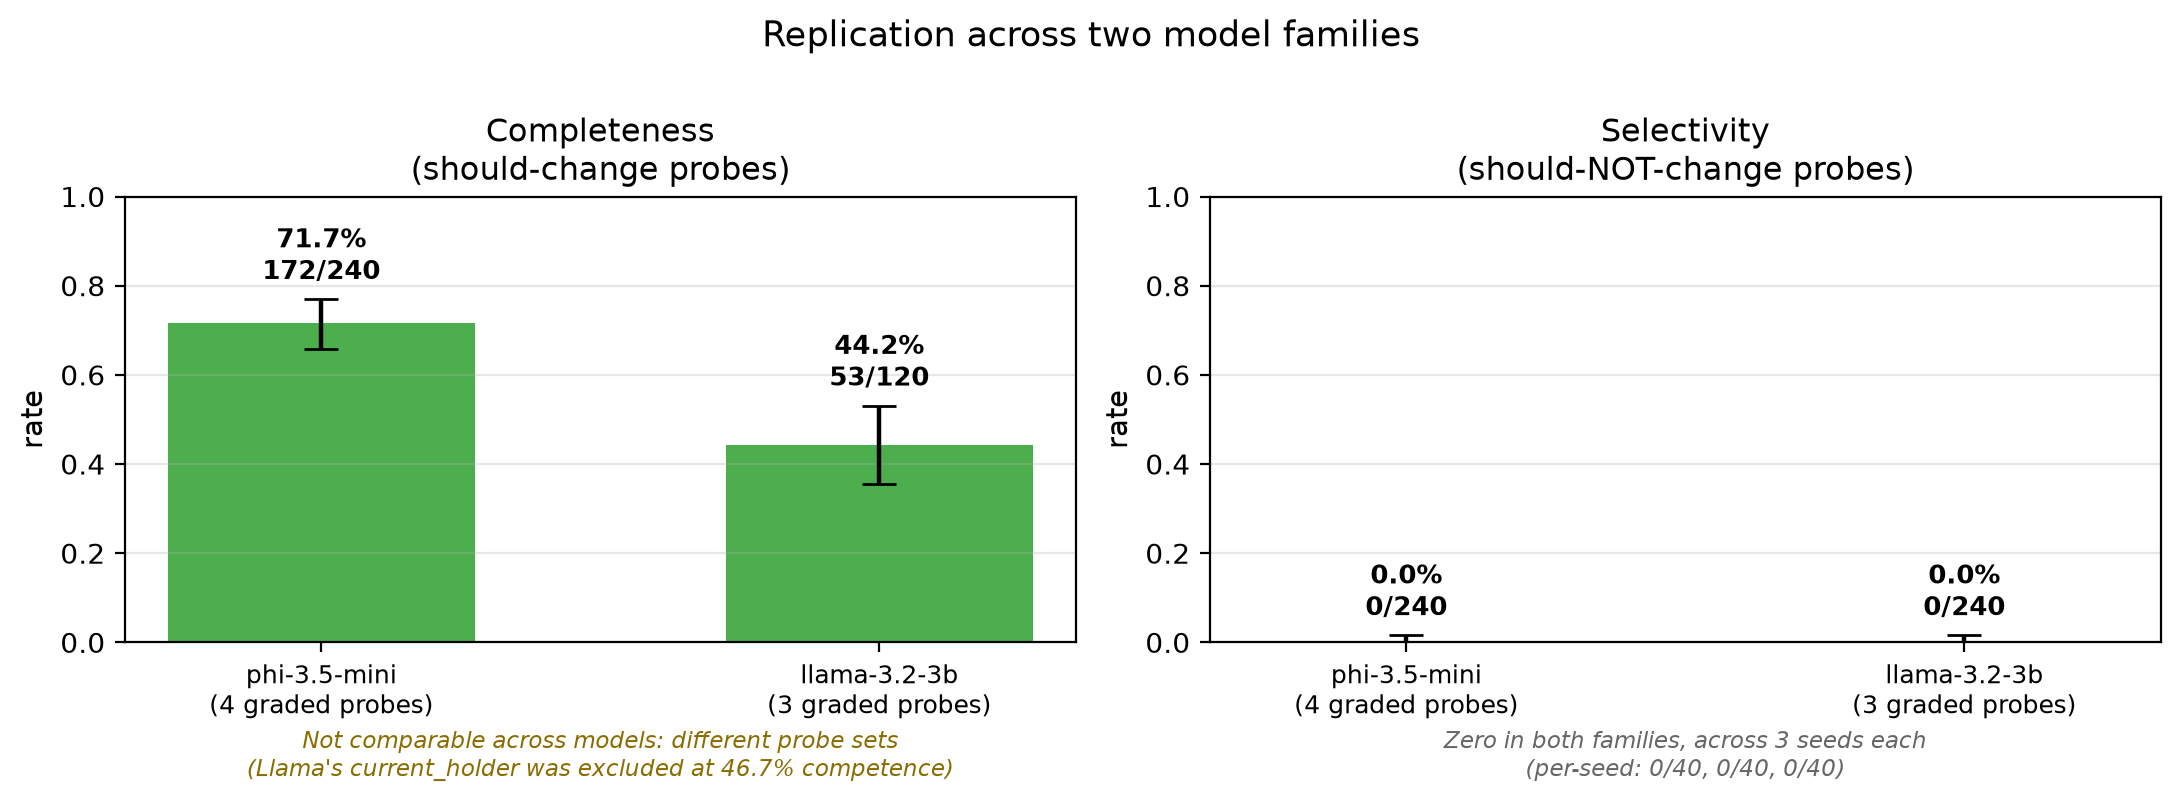
\includegraphics[width=\columnwidth]{fig3_replication.png}
  \caption{Replication across two model families, Wilson 95\% intervals over
    independent pairs. The completeness bars are \emph{not} comparable across
    models: Llama graded three probes to Phi's four, because Llama's
    current-holder probe fell below the competence gate.}
  \label{fig:replication}
\end{figure}

\subsection{Supporting observations}
\label{sec:supporting}

Three observations support the interpretation without being independent
contributions, reported in full in \cref{sec:appendix-supporting}: the effect
is confined to the answer boundary (0/12 transport at positions $-2$ through
$-7$ versus 9/12 at $-1$); compact subspaces do not carry it (0/32 at rank 32
for every basis tested, against 24/32 full-space); and successful edits are
not geometrically diverse, so intervention non-uniqueness does not explain the
failure.

\section{Discussion}
\label{sec:discussion}

\paragraph{What the experiment establishes.}
In this setting, an intervention can satisfy effectiveness, donor specificity,
norm control, and dose-response while exercising no selective control over the
reasoning variable it appears to manipulate. The four credentials are jointly
insufficient. A two-probe consequence check detects this at negligible cost.

\paragraph{What it does not establish.}
It does not show that interchange-intervention accuracy is invalid --- MIB
uses it deliberately to align features with \emph{specified} variables, and
\citet{sutter2025nonlinear} already demonstrate a sharper limitation,
obtaining 100\% IIA on randomly initialized language models with sufficiently
powerful alignment maps. Nor does it show that selective interventions on
reasoning state are impossible; we tested one intervention family at one site.

\paragraph{The obvious objection, conceded.}
One may respond: you patched the final pre-answer token, so of course you
manipulated an answer representation. We agree, and the position sweep is
evidence \emph{for} that reading --- effects appear only where answer
information becomes directly actionable. The point is not that a poorly chosen
site gives a poor result. It is that an intervention at this site passes four
escalating credentials a practitioner would reasonably accept. The credential
stack, not the site, is the object of study.

\paragraph{Relation to prior work.}
RAVEL contributes the effectiveness/selectivity distinction; MIB contributes
its benchmark operationalization and the observation that full-vector
interventions fail it for entity attributes. Our addition is narrow: the same
failure occurs for a \emph{computed} state, and it survives a control battery
considerably stronger than answer-change alone.

\section{Limitations}
\label{sec:limitations}

\begin{enumerate}
  \item \textbf{One task family.} A single transfer-chain task with one causal
    program. We make no claim of universality.
  \item \textbf{Selectivity rests on two probes per model.}
    \texttt{transfer\_count} was excluded in both models (20.8\% and 18.3\%
    competence): neither can count transfers unprompted, so post-intervention
    changes there are uninterpretable.
  \item \textbf{Llama supports only part of the claim.} Its current-holder
    competence is 46.7\% at $n=120$, so its completeness figure is computed on
    a different probe set and is not comparable to Phi's.
  \item \textbf{One intervention site and one layer set.} Layers
    $[18, 20, 22, 24]$ at the final pre-answer position. Other sites may
    behave differently --- indeed \cref{sec:appendix-supporting} shows they
    behave \emph{very} differently.
  \item \textbf{Competence is not shown to drive the effect.} Phi has both
    higher baseline accuracy and stronger intervention takeover, but two
    models cannot establish a relationship between competence and selectivity
    failure. The defensible statement is narrower: the selectivity failure
    cannot be explained by poor baseline task competence, since it persists in
    Phi at 99--100\% baseline accuracy on all graded probes.
  \item \textbf{Small-sample estimates were optimistic.} At $n=24$ Llama's
    current-holder competence appeared to be 88\%; at $n=120$ with freshly
    resampled items it is 46.7\%. Early-stage numbers in this literature,
    including our own, should be treated with caution.
\end{enumerate}

\section{Future work}
\label{sec:future-work}

The sharp dependence on intervention position --- full effect at the final
token, nothing one token earlier --- suggests that selectivity may vary
systematically along the computational trajectory. Mapping where interventions
transition from state-level control to answer-level control, as a grid over
layers and positions with a selectivity panel at each cell, is the natural
next study and a substantially larger undertaking than the present one.

\bibliography{custom}

\appendix

\section{Probe templates and the competence gate}
\label{sec:appendix-probes}

\paragraph{Item construction.}
Each item is a single transfer-chain body (\cref{sec:task}) rendered once and
then queried five ways, so completeness and selectivity are measured on the
\emph{same} underlying problem rather than resampled items per probe. The
donor is always asked the canonical question; only the receiver is asked all
five. The templated slots are filled from the receiver's own problem, never
the donor's, so a probe answered correctly with the \emph{donor's} value
cannot be explained by surface leakage from the question text itself.

\paragraph{Why the competence gate exists.}
A selectivity failure --- a should-not-change probe moving after the patch ---
is only evidence of a semantic leak if the model could answer that probe
correctly \emph{unpatched}. If a model cannot perform the task at all, a
post-intervention \enquote{change} on that probe is noise, not leakage. The
gate is applied per probe, per model, at a 50\% baseline-accuracy floor,
before any selectivity number is computed or reported.

\paragraph{Why \texttt{transfer\_count} was excluded for both models.}
Baseline accuracy was 20.8\% (Phi) and 18.3\% (Llama) --- both models fail to
count transfers unprompted at a rate indistinguishable from guessing among
small integers, independent of any intervention. Reporting a
\enquote{selectivity} result on this probe would conflate task incapacity with
semantic leakage, so it is dropped from the verdict in both models, leaving
four graded probes for Phi and three for Llama.

\paragraph{Answer-token construction.}
Count answers are rendered as words (\enquote{two}, not \enquote{2}), because
the digit form tokenizes inconsistently across architectures --- verified to
silently corrupt generated pairs before being caught. All answers are checked
for single-token status \emph{in the rendered context}, not a naive
leading-space heuristic, since SentencePiece-family tokenizers (Phi) split
some such forms differently.

\section{Supporting observations}
\label{sec:appendix-supporting}

\paragraph{The effect is confined to the answer boundary.}
Patching at positions $-2$ through $-7$ (the queried object, \enquote{the},
\enquote{has}, \enquote{Who}, the sentence-final period, the recipient name)
produces \textbf{0/12} transport for both correct and random donors, while
position $-1$ produces 9/12. There is no intermediate regime in which the
effect is present but weaker.

\paragraph{Compact subspaces do not carry it either.}
At rank 32, projected interchange through tracking, PCA, random,
gradient-coordinate and learned-causal bases all produce 0/32, while the
full-space oracle produces 24/32. Random bases fail at every rank in both
architectures, and PCA performs comparably to a clean-minus-corrupt tracking
basis through the useful rank regime --- evidence that the tracking contrast
does not identify a privileged reasoning subspace.

\paragraph{Successful edits are not geometrically diverse.}
We tested whether behaviorally equivalent edits must be internally similar,
since a negative answer would have offered an alternative explanation for our
results. Across 17 restarts $\times$ 3 examples with randomized
initialization, median pairwise cosine between successful edits is $+0.840$,
$+0.912$, $+0.948$. Solutions travel ${\sim}2.5\times$ their initialization
norm and end nearly orthogonal to their starting points ($\cos \approx 0.02$),
then converge on the same direction regardless. Independently initialized
optimizations find essentially one solution, so intervention non-uniqueness
does not explain the selectivity failure. This also accounts for the low
cosine ($\approx 0.08$--$0.15$) observed between unconstrained and
subspace-confined edits: that is forced by confining a vector to a rank-32
slice of a 3072-dimensional space, not evidence of distinct solutions.

\section{Reproduction}
\label{sec:appendix-reproduction}

All experiments are frozen at a single snapshot; no number in this paper may
be changed without a corresponding change to that snapshot. A verification
script re-checks every quoted number against the frozen logs and fails the
build on any mismatch (44 checks). Item generation, intervention mechanics,
the cross-question panel, donor specificity, the magnitude and position
sweeps, the uniqueness falsification, the selectivity-metric validation, and
all figure generation are each a separate script in the release. Code and
frozen logs will be released upon acceptance.

The panel runs predate an output flag added later and cannot be regenerated
bit-for-bit, since each seed resamples both pairs and prefix; the figure data
is a hand transcription of those logs, and figures are built from it.

\end{document}
